\documentclass{standalone}
\usepackage{amsmath,amssymb,amsthm}
\usepackage{graphicx}
\usepackage[pdfborder= 0 0 0,citecolor=black,linkcolor=black,colorlinks=true,bookmarksopen=true]{hyperref}
\usepackage[notref]{showkeys}
\usepackage{caption}
\usepackage{subcaption}
\usepackage{xcolor}
\usepackage{algorithm}
\usepackage{algorithmicx}
\usepackage{algpseudocode}
\usepackage{tikz}
\usetikzlibrary{positioning}
\usepackage{tikz-3dplot}
\usepackage{gnuplot-lua-tikz}
\usepackage{pgfplots}
\usepackage{authblk}
\usepackage[pagewise]{lineno}
\usepackage{calc}
\usetikzlibrary{plotmarks}
\author[1,*]{P.A. Browne}
\affil[1]{Department of Meteorology, University of Reading, UK}
\affil[*]{Correspondence to p.browne@reading.ac.uk}
\title{EMPIRE comms version 1 and 2}
\makeatletter \AtBeginDocument{ \hypersetup{pdftitle= {\@title},pdfauthor= {\@author}}} \makeatother

\date{\today}


\begin{document}
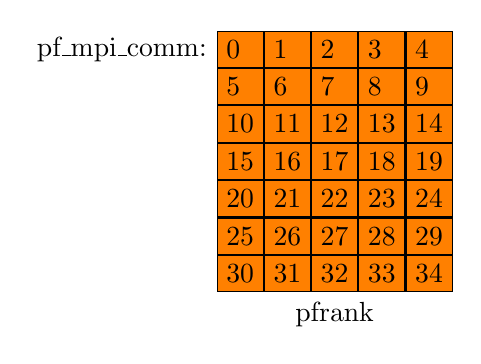
\begin{tikzpicture}[node distance=0em]
\node[fill=orange,draw] (00) at (0,0) {\parbox{\widthof{16}}{0}};
\node[fill=orange,draw,right = of 00] (01) {\parbox{\widthof{16}}{1}};
\node[fill=orange,draw,right = of 01] (02) {\parbox{\widthof{16}}{2}};
\node[fill=orange,draw,right = of 02] (03) {\parbox{\widthof{16}}{3}};
\node[fill=orange,draw,right = of 03] (04) {\parbox{\widthof{16}}{4}};
\node[fill=orange,draw,below= of 00] (10) {\parbox{\widthof{16}}{5}};
\node[fill=orange,draw,right= of 10] (11) {\parbox{\widthof{16}}{6}};
\node[fill=orange,draw,right= of 11] (12) {\parbox{\widthof{16}}{7}};
\node[fill=orange,draw,right= of 12] (13) {\parbox{\widthof{16}}{8}};
\node[fill=orange,draw,right= of 13] (14) {\parbox{\widthof{16}}{9}};
\node[fill=orange,draw,below= of 10] (20) {10};
\node[fill=orange,draw,right= of 20] (21) {11};
\node[fill=orange,draw,right= of 21] (22) {12};
\node[fill=orange,draw,right= of 22] (23) {13};
\node[fill=orange,draw,right= of 23] (24) {14};
\node[fill=orange,draw,below= of 20] (30) {15};
\node[fill=orange,draw,right= of 30] (31) {16};
\node[fill=orange,draw,right= of 31] (32) {17};
\node[fill=orange,draw,right= of 32] (33) {18};
\node[fill=orange,draw,right= of 33] (34) {19};
\node[fill=orange,draw,below= of 30] (40) {20};
\node[fill=orange,draw,right= of 40] (41) {21};
\node[fill=orange,draw,right= of 41] (42) {22};
\node[fill=orange,draw,right= of 42] (43) {23};
\node[fill=orange,draw,right= of 43] (44) {24};
\node[fill=orange,draw,below= of 40] (50) {25};
\node[fill=orange,draw,right= of 50] (51) {26};
\node[fill=orange,draw,right= of 51] (52) {27};
\node[fill=orange,draw,right= of 52] (53) {28};
\node[fill=orange,draw,right= of 53] (54) {29};
\node[fill=orange,draw,below= of 50] (60) {30};
\node[fill=orange,draw,right= of 60] (61) {31};
\node[fill=orange,draw,right= of 61] (62) {32};
\node[fill=orange,draw,right= of 62] (63) {33};
\node[fill=orange,draw,right= of 63] (64) {34};
\node[left = of 00] (pfmpicomm) {pf\_mpi\_comm:};
\node[below = of 62] (title) {pfrank};
\end{tikzpicture}
%\caption{The rank of each process within each communicator}


%\end{figure}
\end{document}
